\documentclass[xcolor=x11names,compress]{beamer}

%% General document %%%%%%%%%%%%%%%%%%%%%%%%%%%%%%%%%%
\usepackage{ucs}     % unicode 
\usepackage[utf8x]{inputenc}  % utf-8
\usepackage[ngerman, english]{babel}  % new german spelling 
\usepackage[T1]{tipa}
\usepackage{ragged2e}
\usepackage{graphicx}
\usepackage{tikz}
\usetikzlibrary{decorations.fractals}
\usepackage{enumitem}
\usepackage{gb4e}
\usepackage{qtree}
\usepackage{soul}
\usepackage{bbding}

%%%%%%%%%%%%%%%%%%%%%%%%%%%%%%%%%%%%%%%%%%%%%%%%%%%%%%


%% Beamer Layout %%%%%%%%%%%%%%%%%%%%%%%%%%%%%%%%%%
\useoutertheme[subsection=false,shadow]{miniframes}
\useinnertheme{default}
\usefonttheme{serif}
\usepackage{palatino}

\setbeamerfont{title like}{shape=\scshape}
\setbeamerfont{frametitle}{shape=\scshape}

\setbeamercolor*{lower separation line head}{bg=DeepSkyBlue4} 
\setbeamercolor*{normal text}{fg=black,bg=white} 
\setbeamercolor*{alerted text}{fg=red} 
\setbeamercolor*{example text}{fg=black} 
\setbeamercolor*{structure}{fg=black} 
 
\setbeamercolor*{palette tertiary}{fg=black,bg=black!10} 
\setbeamercolor*{palette quaternary}{fg=black,bg=black!10} 

\renewcommand{\(}{\begin{columns}}
\renewcommand{\)}{\end{columns}}
\newcommand{\<}[1]{\begin{column}{#1}}
\renewcommand{\>}{\end{column}}
%%%%%%%%%%%%%%%%%%%%%%%%%%%%%%%%%%%%%%%%%%%%%%%%%%


%\documentclass{beamer}
%\usepackage{beamerthemesplit} 
%\usetheme{Goettingen}
%\usecolortheme{seahorse}
\title{Semantic Role Labeling}
\author{Arne Binder, Robert B\"arhold, Enrique Manjavacas}
\date{
	\begin{tikzpicture}[decoration=Koch curve type 2] 
		\draw[DeepSkyBlue4] decorate{ decorate{ decorate{ (0,0) -- (2,0) }}}; 
	\end{tikzpicture}  
	\\
	\vspace{0cm}
	\today
}


\begin{document}

\frame{\titlepage}

\frame{
	\frametitle{Gliederung}
	\tableofcontents
	[pausesections]
}


\section{Theoretischer Hintergrund und Motivation}
	\frame{
		\frametitle{Argumentstruktur von Verben}
		%Beispielverb - zweiseitige Argumentstruktur
	}

	\frame{
		\frametitle{thematische Rollen}
		%Abstraktion über die semantische Seite der Argumentstruktur		
	}

	\frame{
		\frametitle{Frames und Frame elements}
		%Situationsverankerte Abstraktion über die Argumentstruktur
		%Frame element gleich Rolle
		% --> target / praedikat
	}
	
	\frame{
		\frametitle{Motivation}
		%Anwendungsbeispiele 
		%Informationextraktion,...
		%Warum Rollen? theoretisches Beispiel
		%nicht aufschreiben, aber sagen - the linguists scarcity problem, zu viele daten zu wenige linguisten
	}

\section{Problemstellung}

	\frame{
		\frametitle{Problemstellung}
		\centering
		Automatische Bestimmung von Rollen
		%\vspace{1cm} 
		%\fbox{\parbox{\dimexpr \linewidth - 2\fboxrule - 2\fboxsep}{
		\fbox{\parbox{\linewidth}{		
		Lassen sich semantische Rollen anhand von lexikalischen und syntaktischen Informationen eines Satzes automatisch bestimmen?
		}}
		%box rum blauer Rahmen
	}

	\frame{
		\frametitle{Corpus: Salsa 2.0}
		\begin{itemize}
			\item<1->
			Erstellt von der Universität Saarland %Referenz
			\item<2->
			basiert auf dem TIGER-Korpus %Referenz
			\begin{itemize}
				\item<1->
				Treebank über Zeitungsartikel
				\item<2->
				viele syntaktische Informationen:\\ 
				Pos-Tag, morphologische \& lemma-Informationen
			\end{itemize}
			\item<3->
			enthält: ~24.000 Sätze mit 648 Prädikaten %target-word
			\item<4->
			Prädikate: Nomen \& Verben

		\end{itemize}
	%	annotierung genau beschreiben (saetzengrenzen etc...)
	}	
	
	\frame{
		\frametitle{Corpus: Salsa 2.0}
		%Beispielbild von Salt: kurzer Satz mit edge-labels
	}

	
\section{Umsetzung}
	\frame{
		\frametitle{Einschränkungen}

		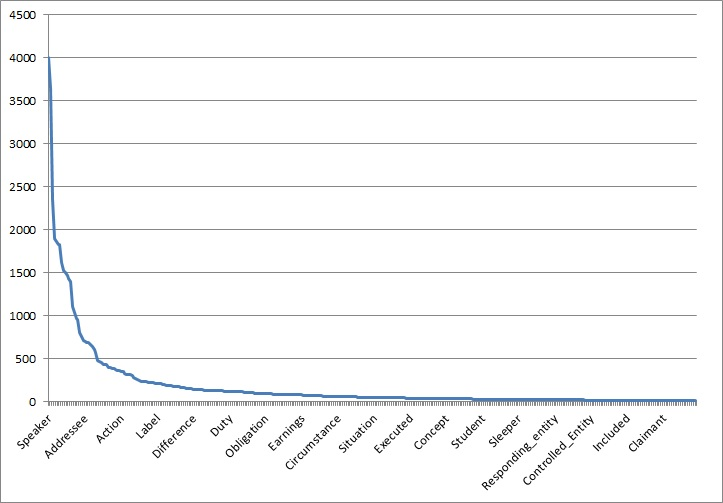
\includegraphics[scale=0.5]{role_frequency.jpg}
	}
	\frame{
		\frametitle{Einschränkungen}
		top 10 rollen
		keine Frames
	}
	
	\frame{
		\frametitle{Herangehensweise}
		Ansatz von jurafsky(und gildea)
		Classifier - naive bayes classifier
		features - anlehnend an jurafsky und gildea (aufzaehlen)
	}
	\frame{
		\frametitle{Probleme}
		Deutsch erlaubt wesentlich freiere Verschiebung von Konstituenten im Satz - Subjekt nicht auf die Vorfeldposition beschr\"ankt....
		Corpusannotation - 
		1. Head nicht \"uberall definiert. Negra Tag Set vorentscheidungen. 
		2. ich ging nach haus' und dr\"uckte die maus (sec-edges)
		3. target identifizieren. gegebenenfalls mehrere woerter
	}
	
	\frame{
		\frametitle{SRL-Ablauf}
		1. Corpus einlesen - aufgeteilt nach Saetzen
		2. interne corpusrepraesentation mit informationen anreichern
		%regelbasiert werden heads gesetzt pfade zum root ermitteln..............
		3. model tranieren [h\"aufigkeiten auszaehlen und normieren]
		%leerzeile
		4. nicht frame annotiertes Corpus einlesen
		5. konstituenten klassifizieren mithilfe des models.
		[6. evaluieren]
	}
	\frame{
		\frametitle{Ablauf des Trainings und der Klassifikation}
		a)Training
		wird alles gezaehlt und target lemmata extrahiert
		b)Klassifikationen
		Satz > Target lemma suchen > alle Konstituenten klassifizieren \& Frame bzg Target lemma speichern
		%smoothing: 0.000001; threshold for frame: P(R1..Rk) > e^(-600)
	}

\section{Evaluieren}
	\frame{
		da wir eine feste liste von target lemmata nutzen und nicht auf ungesehene targets abstrahieren koennen 
		beruecksichtigen wird bei der evaluation nur frame elements mit dem bezug auf ein (im Model) bekanntes target. 
		counts erklaeren und ausgeben 
	}
	\frame{
		\frametitle{Kreuzvalidierung}
		fuenffach plus ergebnisse

	}
	\frame{
		\frametitle{Evaluationsvergleich}
	}









































\frame{
\frametitle{What are semantic  roles?}
\begin{itemize}
	\item<2->
			\begin{xlist}
			\ex
			\gll Peter gibt Karl Geld.\\
			\footnotesize
			\textcolor{blue}{\textit{SOURCE}}
			\footnotesize
			{}
			\footnotesize
			\textcolor{blue}{\textit{RECIPIENT} }
			\footnotesize
			\textcolor{blue}{\textit{THEMA}}
			\\
			\vspace{1cm}
	\item<3->
			
			\gll Karl bekommt Geld von Peter.\\
			\footnotesize
			\textcolor{blue}{\textit{RECIPIENT}}
			\footnotesize
			{}
			\footnotesize
			\textcolor{blue}{\textit{THEMA}}
			\footnotesize
			\textcolor{blue}{\textit{SOURCE}}
			\\
			\end{xlist}

			
\end{itemize}
}



\section[Why Semantic Roles?]{}
\frame{
\frametitle{Why Semantic Roles?}
\begin{itemize}
	\item<1-> \begin{block}{\textbf{Information Extraction}}
	\begin{itemize}
		\item "Paul hat seine Mutter get\"otet."
	\end{itemize}
	\end{block}
	\vspace{1cm}
	\item<2-> \begin{block}{\textbf{Metaphernanalyse}}
	\begin{itemize}
		\item "Paul hat seine Mutter unter die Erde gebracht."
	\end{itemize}
	\end{block}
\end{itemize}
}

\section[Our goal]{}
\frame{
\frametitle{Our goal}
\begin{itemize}
	\item<1-> Automatic Semantic Role Labeling
	\item<2-> Language: German
	\item<3-> Corpus: SALSA 2.0 (based on TIGER Corpus \& FrameNet)
	\item<4-> Framework: LingPipe 
	\vspace{1cm}
	\item<5-> \textbf{References:} C.J. Fillmore (Frame Semantics), D. Jurafsky \& D. Gildea (first implementation of a Semantic Role Labeler)
	
\end{itemize}
}



\end{document}
